% arara: xelatex
\documentclass[12pt]{article}

% \usepackage{physics}

\usepackage{hyperref}
\hypersetup{
    colorlinks=true,
    linkcolor=blue,
    filecolor=magenta,      
    urlcolor=cyan,
    pdftitle={Overleaf Example},
    pdfpagemode=FullScreen,
    }

\usepackage{tikzducks}

\usepackage{tikz} % картинки в tikz
\usetikzlibrary{shapes, arrows, positioning}
\usepackage{microtype} % свешивание пунктуации

\usepackage{array} % для столбцов фиксированной ширины

\usepackage{indentfirst} % отступ в первом параграфе

\usepackage{sectsty} % для центрирования названий частей
\allsectionsfont{\centering}

\usepackage{amsmath, amsfonts, amssymb} % куча стандартных математических плюшек

\usepackage{comment}

\usepackage[top=2cm, left=1.2cm, right=1.2cm, bottom=2cm]{geometry} % размер текста на странице

\usepackage{lastpage} % чтобы узнать номер последней страницы

\usepackage{enumitem} % дополнительные плюшки для списков
%  например \begin{enumerate}[resume] позволяет продолжить нумерацию в новом списке
\usepackage{caption}

\usepackage{url} % to use \url{link to web}

\usepackage{xcolor}   % для цвета текста
\usepackage{ulem}     % для зачёркивания (\sout)

\usepackage[symbol]{footmisc}

\newcommand{\smallduck}{
\begin{tikzpicture}[scale=0.3]
    \duck[
        cape=black,
        hat=black,
        mask=black
    ]
    \end{tikzpicture}}

\usepackage{fancyhdr} % весёлые колонтитулы
\pagestyle{fancy}
\lhead{Stochastic Processes}
\chead{}
\rhead{Black Midterm, retake}
\lfoot{}
\cfoot{}
\rfoot{}

\renewcommand{\headrulewidth}{0.4pt}
\renewcommand{\footrulewidth}{0.4pt}

\usepackage{tcolorbox} % рамочки!

\usepackage{todonotes} % для вставки в документ заметок о том, что осталось сделать
% \todo{Здесь надо коэффициенты исправить}
% \missingfigure{Здесь будет Последний день Помпеи}
% \listoftodos - печатает все поставленные \todo'шки


% более красивые таблицы
\usepackage{booktabs}
% заповеди из докупентации:
% 1. Не используйте вертикальные линни
% 2. Не используйте двойные линии
% 3. Единицы измерения - в шапку таблицы
% 4. Не сокращайте .1 вместо 0.1
% 5. Повторяющееся значение повторяйте, а не говорите "то же"


\setcounter{MaxMatrixCols}{20}
% by crazy default pmatrix supports only 10 cols :)


\usepackage{fontspec}
\usepackage{libertine}
\usepackage{polyglossia}

\setmainlanguage{russian}
\setotherlanguages{english}


\usetikzlibrary{automata, positioning, arrows.meta, calc, shapes.multipart}


% download "Linux Libertine" fonts:
% http://www.linuxlibertine.org/index.php?id=91&L=1
% \setmainfont{Linux Libertine O} % or Helvetica, Arial, Cambria
% why do we need \newfontfamily:
% http://tex.stackexchange.com/questions/91507/
% \newfontfamily{\cyrillicfonttt}{Linux Libertine O}

\AddEnumerateCounter{\asbuk}{\russian@alph}{щ} % для списков с русскими буквами
% \setlist[enumerate, 2]{label=\asbuk*),ref=\asbuk*}

%% эконометрические сокращения
\DeclareMathOperator{\Cov}{\mathbb{C}ov}
\DeclareMathOperator{\Corr}{\mathbb{C}orr}
\DeclareMathOperator{\Var}{\mathbb{V}ar}
\DeclareMathOperator{\col}{col}
\DeclareMathOperator{\row}{row}

\let\P\relax
\DeclareMathOperator{\P}{\mathbb{P}}

\DeclareMathOperator{\E}{\mathbb{E}}
% \DeclareMathOperator{\tr}{trace}
\DeclareMathOperator{\card}{card}

\DeclareMathOperator{\Convex}{Convex}
\DeclareMathOperator{\plim}{plim}

\newcommand{\cN}{\mathcal{N}}
\newcommand{\cF}{\mathcal{F}}

\newcommand{\RR}{\mathbb{R}}
\newcommand{\NN}{\mathbb{N}}
\newcommand{\hb}{\hat{\beta}}
\newcommand{\dPois}{\mathrm{Pois}}
\newcommand{\dUnif}{\mathrm{Unif}}
\newcommand{\dExpo}{\mathrm{Expo}}





\begin{document}

\textcolor{red}{\textbf{FINAL SALE}}: Every problem will bring you 10 \sout{99.99} points!

Scratch paper price: \sout{10 points per sheet only} \textcolor{red}{\textbf{FREE\footnote[1]{Members only deal!}}}!

\begin{enumerate}
    \item Dragon Erik has three towns to kidnap a princess from: $A$, $B$ and $C$.
    He kidnaps the first princess from town $A$ and chooses every next town according to a Markov chain with transition matrix $T$,
    where states are written in alphabetical order:
    \[
    T = \begin{pmatrix}
        0.2 & 0.1 & ? \\
        ? &  0 & 0.6 \\
        0.5 & ? & 0.3 \\
    \end{pmatrix}.
    \]
    \begin{enumerate}
        \item {[2]} Fill in the missing values. 
        \item {[2]} Draw the graph of the Markov chain. 
        \item {[3]} What is the probability that the third princess will be from town $B$?
        \item {[3]} What is the probability that the second princess was from $A$ given that the third princess was from $B$?
    \end{enumerate}


    \item Every minute the cat Tikhon says «meow» with probability $1/3$ or «purr» with probability $2/3$ independently of all other words.
    
    Let $T$ be the first moment of time when he says the sequence «meow-purr-meow». 
    \begin{enumerate}
        \item {[5]} Find $\E(T)$.
        \item {[5]} Find $\Var(T)$.
    \end{enumerate}

    \item {[10]} Gumbatali starts with zero initial sum $S_0 = 0$. 
    Every minute he either wins $X_t = 1$ dollar with probability $1/4$ or pays $1$ dollar, $X_t = -1$, with probability $3/4$.
    He can't go neither below $S_t = -3$ nor above $S_t = 2$, so that
    \[
    S_t = \min\{2, \max\{-3, S_{t-1} + X_t\}\}.
    \]
    The random variables $(X_t)$ are independent. 
    
    Find the stationary distribution of $S_t$.


\newpage
\item Consider the Markov chain:

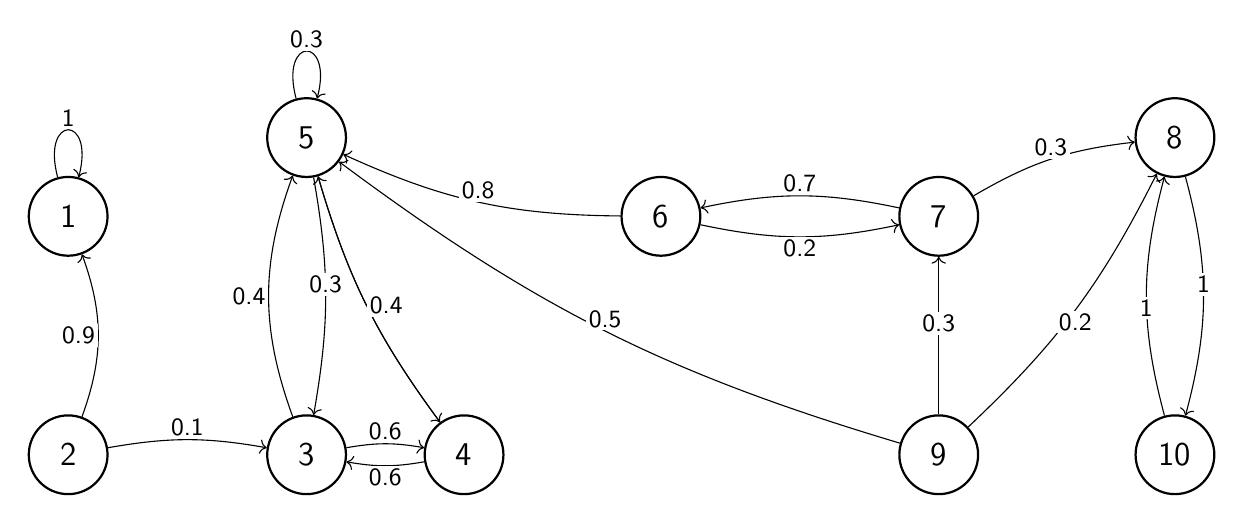
\begin{tikzpicture}[
    node distance=50mm,
    state/.style={circle, draw=black, thick, minimum size=10mm, inner sep=1pt, font=\sffamily\large},
    every edge/.style={->, >=Stealth, semithick},
    lab/.style={fill=white, inner sep=1pt, font=\sffamily\small}
]

% --- nodes (arranged for a clear diagram) ---
\node[state] (2)  {2};
% absorbing
\node[state, above=20mm of 2] (1)  {1};

% closed class A member
\node[state, right=20mm of 2] (3) {3}; 
% closed class A member (loop)
\node[state, above=30mm of 3] (6) {5};  
 % closed class A member
\node[state, right=40mm of 2] (9) {4};           

% periodic closed class (small 2-cycle)
\node[state, right=100mm of 6] (4) {8};
\node[state, below=30mm of 4] (5) {10};

% transient / connector states on right
\node[state, right=70mm of 3] (7) {9};
\node[state, above=20mm of 7] (10) {7};
\node[state, left=25mm of 10] (11) {6};

% --- edges with probabilities ---
% state 1: absorbing
\draw[->] (1) to [loop above] node[lab] {1} ();

% state 2: transient -> 1 and -> 3
\draw[->] (2) to[bend right=20] node[lab, left] {0.9} (1);
\draw[->] (2) to[bend left=10] node[lab, above] {0.1} (3);

% closed class A: nodes 3,6,9 (aperiodic because 6 has self-loop)
\draw[->] (3) to[bend left=20] node[lab, left] {0.4} (6);
\draw[->] (3) to[bend left=10] node[lab, above] {0.6} (9);

\draw[->] (6) to[bend left=10] node[lab, above] {0.3} (3);
\draw[->] (6) to[bend right=10] node[lab, below] {} (9);
\draw[->] (6) to[loop above] node[lab] {0.3} ();

\draw[->] (9) to[bend left=10] node[lab, below] {0.6} (3);
\draw[->] (9) to[bend left=10] node[lab, right] {0.4} (6);

% periodic closed class (2-cycle): 4 <-> 5 (period 2)
\draw[->] (4) to[bend left=15] node[lab, above] {1} (5);
\draw[->] (5) to[bend left=15] node[lab, below] {1} (4);

% transient connectors on right
% to closed A
\draw[->] (7) to[bend left=10] node[lab, above] {0.5} (6);  
% to periodic closed class
\draw[->] (7) to[bend right=10] node[lab, below] {0.2} (4);  
% to transient 10
\draw[->] (7) to node[lab, above] {0.3} (10);               

% state 10: transient (flows to closed class 4 or to 11)
\draw[->] (10) to[bend left=12] node[lab, above] {0.3} (4);
\draw[->] (10) to[bend right=12] node[lab, above] {0.7} (11);

% state 11: transient (feeds back toward closed A or to 10)
\draw[->] (11) to[bend left=12] node[lab, above] {0.8} (6);
\draw[->] (11) to[bend right=12] node[lab, below] {0.2} (10);

\end{tikzpicture}

\begin{enumerate}
    \item {[5]} Using a chainsaw
    %\footnote[1]{We have excellent discounts on chainsaws today!} 
    cut the Markov chain into communicating classes and classify them as transient, positive recurrent or null-recurrent.
    \item {[1]} Is the chain irreducible?
    \item {[4]} Find the period of every state.
\end{enumerate}


    \item Let \( X \) be exponentially distributed random variable with intensity \( \lambda = 2 \).  
The density for $x\geq 0$ is given by:
\[
f(x) = \lambda \exp(-\lambda x).
\]

\begin{enumerate}
    \item {[4]} Derive the moment generating function \( M_X(t) = \E(e^{tX})\).
    \item {[3]} Using moment generating function find the mean and variance of \(X\).
    \item {[3]} Let \( X_1 \sim \dExpo(\lambda = 2) \) and \( X_2 \sim \dExpo(\lambda = 3) \) be independent random variables. 
    Find the moment generating function of \( S = X_1 + X_2 \). Is $S$ exponentially distributed?
\end{enumerate}

\item By the mayor's decree, the city installs $T_n$ New Year's trees each day, \( n = 1, 2, \ldots \), starting from October 20th. 
The random variables $T_1, T_2, \dots$ are independent and take any natural value from $0$ to $4$ with equal probabilities. 

The amounts of snow $(W_n)$ are independent and uniformly distributed on $[0; 2/n]$. 

Determine the probability limits for the following sequences:
\begin{enumerate}
    \item {[2]} mayor's New Year kpi,   
    \(    X_n = \frac{1}{n} \sum_{i=1}^n T_i
    \)
    \item {[3]} the New Year's mood given by
    \(
    Y_n = \frac{2 X_n +1}{X_n + 10}
    \)
    \item {[5]} The average number of snowmen that can be built each day:
    \(
    S_n = \frac{1}{n} \sum_{i=1}^n W_i^2.
    \)
\end{enumerate}

\end{enumerate}


\end{document}

